\documentclass[a4paper, onecolumn]{article}
\usepackage{lipsum}
\usepackage{graphicx}
\usepackage{tikz}
\usetikzlibrary{quotes,arrows.meta}

\usetikzlibrary{3d} %for including external image 
\usetikzlibrary{positioning}
\usetikzlibrary{shapes.geometric}
\usetikzlibrary{automata}
\usetikzlibrary{angles, quotes}
\usetikzlibrary{arrows,decorations.pathmorphing,backgrounds,positioning}

\definecolor{echoreg}{HTML}{2cb1e1}
\definecolor{olivegreen}{rgb}{0,0.6,0}
\definecolor{mymauve}{rgb}{0.58,0,0.82}


\usepackage{Ball}

\usepackage{etoolbox}

\newtoggle{redraw}
\newtoggle{redraw2}


\title{work with Tikz}
\author{meysam}

\def\SumColor{rgb:blue,5;green,15}



\begin{document}
	\maketitle	
	
	\begin{abstract}
		\lipsum[1]
	\end{abstract}
	
	\tableofcontents
	
	\section{Introduction}
	\lipsum[1-5]
	
	\section{Figures}\label{sect:figures}
	\lipsum[1-3]
	\section{Tikz}
	
	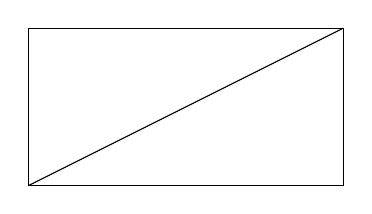
\begin{tikzpicture}[scale=10]
		\draw (0.0,0.0) rectangle (0.4,0.2);
		\draw (0.0,0.0) -- (0.4,0.2);
	\end{tikzpicture}\\
	\lipsum[1-3]
	\begin{figure}
		\centering
		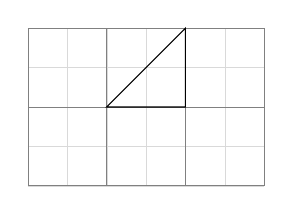
\begin{tikzpicture}
			\draw[line width=0.1pt,gray!30,step=5mm]
			(0,0) grid (3,2);
			\draw[help lines] (0,0) grid (3,2);
			\draw (1,1) -- (2,2) -- (2,1) -- cycle;
		\end{tikzpicture}
		\caption{Tikz Plot}
	\end{figure}

	\lipsum[1-3]
	

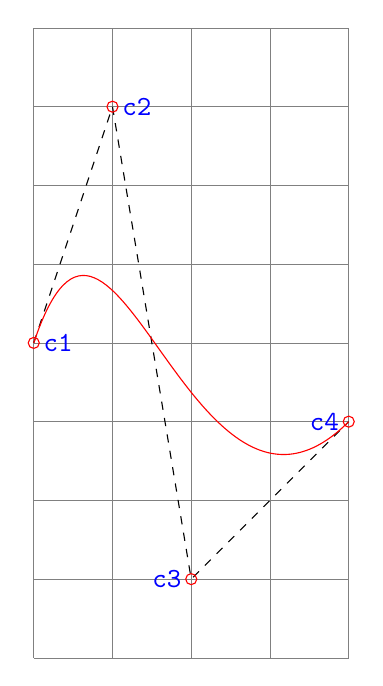
\begin{tikzpicture}
	\draw[help lines] (-2,-4) grid (+2,+4);
	\path (-2,+0) coordinate(c1)
	(-1,+3) coordinate(c2)
	(+0,-3) coordinate(c3)
	(+2,-1) coordinate(c4);
	\draw[dashed] (c1) -- (c2) -- (c3) -- (c4);
	\draw [color=red] (c1) circle (2pt)
	(c2) circle (2pt)
	(c3) circle (2pt)
	(c4) circle (2pt)
	(c1) .. controls (c2)
	and (c3) .. (c4);
	\draw [color=blue]
	(c1) node[anchor=west] {\texttt{c1}}
	(c2) node[anchor=west] {\texttt{c2}}
	(c3) node[anchor=east] {\texttt{c3}}
	(c4) node[anchor=east] {\texttt{c4}};
	
\end{tikzpicture}

	\lipsum[1]
	
	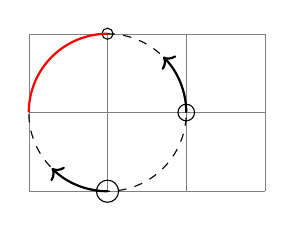
\begin{tikzpicture}
		\draw[help lines] (0,0) grid (3,2);
		\draw[dashed] (1,1) circle (1cm);
		\draw (1,2) coordinate(a) circle (2pt)
		(2,1) coordinate(b) circle (3pt)
		(1,0) coordinate(c) circle (4pt);
		\draw[color=red,-,thick] (a) arc (90:180:1cm);
		\draw[->,thick] (b) arc (0:45:1cm);
		\draw[->,thick] (c) arc (270:225:1cm);
	\end{tikzpicture}
	
	
	
	\lipsum[1]
	\subsection{Colour}
	\begin{tikzpicture}[color=red]
		\draw (0,3) -- (2,3);
		\draw[color=green, thick, ->] (0,2) -- (2,2);
		\draw[color=cyan!50!red] (0,1) -- (2,1);
	\end{tikzpicture}


\lipsum[1]


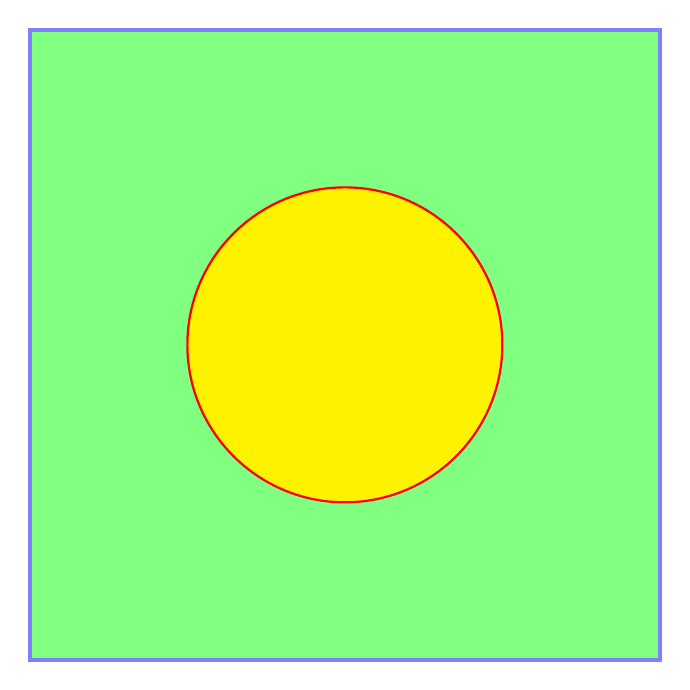
\begin{tikzpicture}[fill=blue!40,scale=4]
	\filldraw[ultra thick,fill=green!50, draw=blue!50]
	(0,0) rectangle (2,2);
	\filldraw[thick,fill=yellow,draw=red]
	(1,1) circle (0.5cm);
\end{tikzpicture}

\lipsum[1]

\tikzset{%
	pics/cube/.style args={#1/#2/#3/#4}{code={%
			\begin{scope}[line width=#4mm]
				\begin{scope}
					\clip (-#1,-#2,0) -- (#1,-#2,0) -- (#1,#2,0) -- (-#1,#2,0) -- cycle;
					\filldraw (-#1,-#2,0) -- (#1,-#2,0) -- (#1,#2,0) -- (-#1,#2,0) -- cycle;
				\end{scope}
				\iftoggle{redraw}{%
				}{%
					\begin{scope}
						\clip (-#1,-#2,0) -- (-#1-#3,-#2,-#3) -- (-#1-#3,#2,-#3) -- (-#1,#2,0) -- cycle;
						\filldraw (-#1,-#2,0) -- (-#1-#3,-#2,-#3) -- (-#1-#3,#2,-#3) -- (-#1,#2,0) -- cycle;
					\end{scope}
				}
				\iftoggle{redraw2}{%
				}{
					\begin{scope}
						\clip (-#1,#2,0) -- (-#1-#3,#2,-#3) -- (#1-#3,#2,-#3) -- (#1,#2,0) -- cycle;
						\filldraw (-#1,#2,0) -- (-#1-#3,#2,-#3) -- (#1-#3,#2,-#3) -- (#1,#2,0) -- cycle;
					\end{scope}
				}
				\node[inner sep=0] (-A) at (-#1-#3*0.5, 0, -#3*0.5) {};
				\node[inner sep=0] (-B) at (#1-#3*0.5, 0, -#3*0.5) {};
				
				\coordinate (-V) at (#1, #2);
				\coordinate (-W) at (#1, -#2);
			\end{scope}
}}}


  \def\r{3}
  

\begin{tikzpicture}
	\tikzstyle{connection}=[ultra thick,every node/.style={sloped,allow upside down},draw=\edgecolor,opacity=0.7]
	\node[canvas is zy plane at x=0] (temp) at (-3,0,0)
	 {
\includegraphics[width=2cm,height=2cm]{1_1_09_2f_37.png}};
	
	\draw [color=black]
	 (temp) node[anchor=south] at (-3,-2){\texttt{Input Face}};
	%\draw[connection] 
	\draw[->,thick] (-2.5,0) -- (-2,0);
	
	\node[trapezium,
	draw = blue!80,
	text = black,
	fill = teal!20,
	rotate=270,
	trapezium stretches = true,
	minimum width = 2cm, 
	minimum height = 3cm] (t) at (-.5,0) {Feature Extraction};
	
	\draw[->,thick] (1.2,0) -- (1.7,0);
	
	\pic[fill=red!50] (FF) at (2.2,0) {cube={0.25/1/0.25/0.1}};
	
	% \draw [color=black ,]
	% node[anchor=south] at (2.2,-2){\texttt{\small Feature Vector}};
	
	\node[color=black, rotate=270,] at (2.2,0) {\small
		 Feature Vector};
	
	\draw[->,thick] (2.5,0) -- (3,0);
	
	
	\node[rectangle,
	draw = magenta!80,
	text = black,
	fill = magenta!20,
	rotate=270,
	trapezium stretches = true,
	minimum width = 1cm, 
	minimum height = 1.5cm] (t) at (3.8,0) {Classification};
	
	\draw[->,thick] (4.5,0) -- (5,0);
	\node[circle,
	draw=brown,
	text=white,
	fill=lightgray] (c) at (6,0){0/1};

		
\end{tikzpicture}




\lipsum

\begin{tikzpicture}
\tikzstyle{connection}=[ultra thick,every node/.style={sloped,allow upside down},draw=\edgecolor,opacity=0.7]
\node[canvas is zy plane at x=0] (temp) at (-3,0,0)
{
\includegraphics[width=2cm,height=2cm]{1_1_09_2f_37.png}};

\draw [color=black]
(temp) node[anchor=south] at (-3,-2){\texttt{Input Face}};
%\draw[connection] 
\draw[->,thick] (-2.5,0) -- (-2,0);

\node[rectangle,
draw = orange!80,
text = black,
fill = orange!20,
rotate=270,
trapezium stretches = true,
minimum width = 3cm, 
minimum height = 0.75cm] (t) at (-2.5,0) {$LBP_{tr}$};

\node[trapezium,
draw = blue!80,
text = black,
fill = teal!20,
rotate=270,
trapezium stretches = true,
minimum width = 2cm, 
minimum height = 3cm] (t) at (-.5,0) {EfficientNet B0};

\draw[->,thick] (1.2,0) -- (1.7,0);

\pic[fill=red!20] (FF) at (2.2,0) {cube={0.25/1.2/0.25/0.1}};

% \draw [color=black ,]
% node[anchor=south] at (2.2,-2){\texttt{\small Feature Vector}};

\node[color=black, rotate=270,] at (2.2,0) {\small
	Feature Vector};

\draw[->,thick] (2.5,0) -- (3,0);


\node[rectangle,
draw = magenta!80,
text = black,
fill = magenta!20,
rotate=270,
trapezium stretches = true,
minimum width = 1cm, 
minimum height = 1.5cm] (t) at (3.8,0) {Classification};

\draw[->,thick] (4.5,0) -- (5,0);
\node[circle,
draw=brown,
text=white,
fill=lightgray] (c) at (6,0){0/1};


\end{tikzpicture}


\lipsum[1]

\begin{tikzpicture}

% Define radius
\def\r{3}

% Bloch vector
\draw (0, 0) node[circle, fill, inner sep=1] (orig) {};
% Sphere


% Axes
\draw[->] (orig) -- ++(-\r/5, -\r/3) node[below] (x1) {$x_1$};
\draw[->] (orig) -- ++(\r, 0) node[right] (x2) {$x_2$};
\draw[->] (orig) -- ++(0, \r) node[above] (x3) {$x_3$};



\end{tikzpicture}

\lipsum[1]



\begin{tikzpicture}

\node (1) [draw, dashed, minimum height=15em, minimum width=62em, xshift=24em, fill=olivegreen, fill opacity=0.2, very thick, rectangle, rounded corners] {};
\node (la1) [below=0em of 1] {{\emph{encoder}}};
\node (2) [draw, dashed, minimum height=14em, fill = red, fill opacity=0.2,minimum width=35em, xshift=63.5em, very thick, rectangle, rounded corners] {};
\node (la1) [below=0em of 2] {{\emph{decoder}}};

\node[] (i2) {};
\pic[fill=green!50] (I2) {cube={1.8/1.8/0.4/1}};

\togglefalse{redraw}
\togglefalse{redraw2}

\node[right=16em of i2] (y) {};

\pic[right=16em of i2, fill=echoreg!50] (Y) {cube={1.8/1.8/1/1}};

\node[right=12em of y] (y1) {};
\pic[right=12em of y, fill=red!50] (Y1) {cube={0.9/0.9/1/1}};

\node[right=12em of y1] (y2) {};
\pic[right=12em of y1, fill=echoreg!50] (Y2) {cube={0.9/0.9/2/1}};
\node[right=10em of y2] (y3) {};
\pic[right=10em of y2, fill=red!50] (Y3) {cube={0.45/0.45/2/1}};

\node[right=9em of y3] (z1) {};
\pic[right=9em of y3, fill=mymauve!50] (Z1) {cube={0.9/0.9/1/1}};

\node[right=12em of z1] (z2) {};
\pic[right=12em of z1, fill=mymauve!50] (Z2) {cube={1.8/1.8/0.4/1}};

\draw [-stealth, ultra thick] (I2-B) -- node[above] {Conv.} node[below] {ReLU} (Y-A);

\draw [-stealth, ultra thick] (Y-B) -- node[above] {Pool} (Y1-A);

\draw [-stealth, ultra thick] (Y1-B) -- node[above=0.3em, inner sep=0.1em] {Conv.} node[below] {ReLU} (Y2-A);

\draw [-stealth, ultra thick] (Y2-B) -- node[above] {Pool} (Y3-A);


\draw [-stealth, ultra thick] (Y3-B) -- node[above] {Deconv.} node[below] {ReLU} (Z1-A);

\draw [-stealth, ultra thick] (Z1-B) -- node[above] {Deconv.} node[below] {logistic} (Z2-A);


\color{black}

\toggletrue{redraw}
\toggletrue{redraw2}

\node[right=16em of i2] (y) {};
\pic[right=16em of i2, fill=echoreg!50] (Y) {cube={1.8/1.8/1/1}};

\pic[right=12em of y, fill=red!50] (Y1) {cube={0.9/0.9/1/1}};

\pic[right=12em of y1, fill=echoreg!50] (Y2) {cube={0.9/0.9/2/1}};

\pic[right=9em of y3, fill=mymauve!50] (Z1) {cube={0.9/0.9/1/1}};

\togglefalse{redraw2}

\pic[right=10em of y2, fill=red!50] (Y3) {cube={0.45/0.45/2/1}};

\toggletrue{redraw2}

\node[] (i2) {\LARGE ${\bf X}$};
\node[right=9.25em of y2] (y3) {\LARGE ${\bf z}$};
\node[right=11em of z1] (z2) {\LARGE ${\bf X}'$};

\end{tikzpicture}









	
	
\end{document}
















